\documentclass[11pt,a4paper]{article}
\usepackage[utf8]{inputenc}\usepackage[T1]{fontenc}
\usepackage[margin=0.9in]{geometry}
\usepackage{amsmath,amssymb,booktabs,graphicx,enumitem,xcolor,parskip,titlesec}
\usepackage[hidelinks]{hyperref}
\graphicspath{{figures/}}
\definecolor{qnavy}{RGB}{20,40,75}\definecolor{qgrey}{RGB}{90,90,90}\definecolor{qred}{RGB}{150,30,30}
\definecolor{qgreen}{RGB}{47,107,79}
\titleformat{\section}{\large\bfseries\color{qnavy}}{\thesection}{0.6em}{}
\begin{document}\thispagestyle{empty}
\noindent
{\large\bfseries\color{qnavy} Report R24 --- Does Epigenetic Modulation Reverse the Drug-Resistance
Programme?}\\[2pt]
{\color{qgrey}SMARCA4 knockdown in osimertinib-resistant lung cancer cells. The knockdown worked.
The reversal was partial in one direction only, and it did not replicate.}\\[6pt]
{\color{qgrey}\rule{\textwidth}{0.4pt}}

\medskip
\noindent 20 August 2026 \quad\textbullet\quad Quantara \quad\textbullet\quad
{\color{qgrey}Peer-review audit copy}

\section*{Summary}

SMARCA4 (BRG1) is the ATPase of the SWI/SNF chromatin remodelling complex, so knocking it down in
an osimertinib-resistant cell line \emph{is} epigenetic modulation of a resistant state. That makes
``reprogramming drug resistance through epigenetic modulation'' a testable claim rather than an
assertion, and GSE202859 contains the experiment: three parental/resistant pairs plus SMARCA4 shRNA
knockdown in two resistant models.

The analysis plan was SHA-256 hashed at \texttt{bffbaad89936c522\ldots} after reading only the TPM
column headers and \emph{before any expression value was compared between any two groups}.

\textbf{Verdict: PARTIAL\_one\_direction\_only}, by the plan's own rule. Reversal required
resistance-UP genes to fall below the null \emph{and} resistance-DOWN genes to rise above it. The
first happened; the second did not. In the second model the whole pattern inverts.

\begin{center}
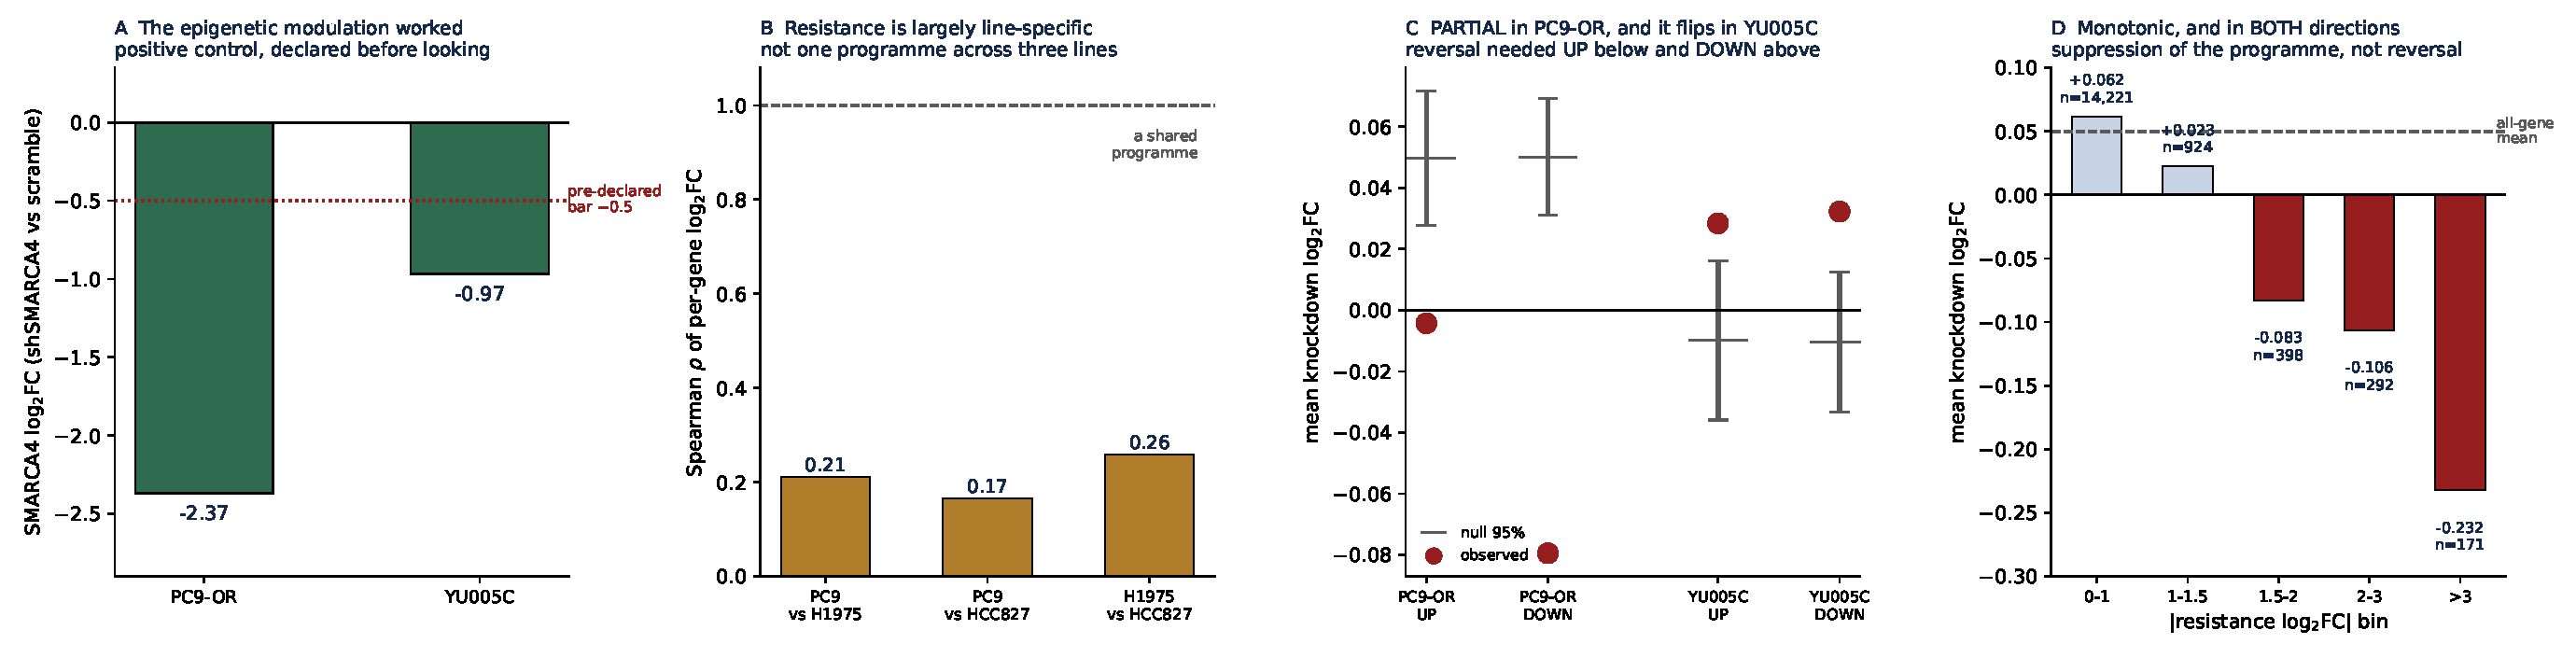
\includegraphics[width=\textwidth]{r24_panels.pdf}
\end{center}
\noindent{\small\color{qgrey}\textbf{A} Knockdown verification. \textbf{B} Cross-line consistency
of the resistance programme. \textbf{C} The primary test in both models. \textbf{D} Knockdown
response by magnitude of resistance change.}

\section{What was measured}

\textbf{The knockdown worked, comfortably.} SMARCA4 log$_2$FC $\mathbf{-2.37}$ in PC9-OR and
$-0.97$ in YU005C, against a pre-declared bar of $-0.5$. This was a gate: had it failed, the plan
required halting without interpreting anything downstream.

\textbf{Resistance changes the transcriptome.} 1{,}785, 1{,}480 and 2{,}367 genes at
$|\log_2\text{FC}| > 1$ in PC9, H1975 and HCC827 respectively, from 16{,}006 retained genes.

\textbf{But the resistance programme is largely line-specific.} Pairwise Spearman correlation of
per-gene log$_2$FC between the three lines is only \textbf{0.17--0.26}. A programme shared across
EGFR-mutant lines would sit near 1. This bears directly on the premise that there is \emph{a}
resistance programme to reprogramme.

\subsection{The primary test}

Resistance sets were defined from the PC9 parental pair alone --- 789 up, 996 down --- so the sets
never touch a knockdown sample. Knockdown log$_2$FC was then compared against 2{,}000 random gene
sets of matched size.

\begin{center}
\begin{tabular}{@{}lrrrl@{}}
\toprule
\textbf{Model / set} & \textbf{$n$} & \textbf{mean kd log$_2$FC} & \textbf{null 95\%} &
\textbf{reading} \\
\midrule
PC9-OR, resistance UP & 789 & $-0.0043$ & $[+0.028, +0.072]$ & below null --- \emph{reversal} \\
PC9-OR, resistance DOWN & 996 & $-0.0795$ & $[+0.031, +0.069]$ & below null --- \emph{not} reversal \\
\midrule
YU005C, resistance UP & 789 & $+0.0284$ & $[-0.036, +0.016]$ & above null --- opposite \\
YU005C, resistance DOWN & 996 & $+0.0322$ & $[-0.033, +0.012]$ & above null --- opposite \\
\bottomrule
\end{tabular}
\end{center}

All four are separable from their nulls at $p \leq 0.004$. What they are not is a reversal:
knockdown pushes resistance-associated genes \emph{down in both directions} in PC9-OR, and up in
both directions in YU005C.

\subsection{One clean finding}

Binning genes by how much they changed on becoming resistant:

\begin{center}
\begin{tabular}{@{}lrr@{}}
\toprule
\textbf{$|$resistance log$_2$FC$|$} & \textbf{$n$} & \textbf{mean knockdown log$_2$FC} \\
\midrule
0--1 & 14{,}221 & $+0.062$ \\
1--1.5 & \phantom{0}\phantom{0}924 & $+0.023$ \\
1.5--2 & \phantom{0}\phantom{0}398 & $-0.083$ \\
2--3 & \phantom{0}\phantom{0}292 & $-0.106$ \\
$>3$ & \phantom{0}\phantom{0}171 & $\mathbf{-0.232}$ \\
\bottomrule
\end{tabular}
\end{center}

Monotonic across five bins: the more a gene changed on becoming resistant, the more SMARCA4
knockdown lowers it. That is a real dose-dependent relationship and it is the most interesting
number in the report --- but it operates on resistance-associated genes regardless of \emph{which
way} they moved, which is suppression of the programme rather than reversal of it.

\section{Why the honest reading is weak}

\textbf{Effect sizes are minute.} $-0.004$ to $-0.079$ log$_2$FC. Statistically separable from a
2{,}000-permutation null, biologically close to nothing.

\textbf{It does not replicate.} YU005C inverts every sign. One model showing partial reversal and a
second showing the opposite is not a finding about SMARCA4; it is two observations that disagree.

\textbf{The premise is shakier than the result.} With cross-line consistency at 0.17--0.26, ``the
resistance programme'' is not one thing across EGFR-mutant lines, so a therapy that reprogrammes
\emph{it} has an ill-defined target.

\section{Limitations}

\textbf{Two to three replicates per group.} This is a small experiment and no negative-binomial
count model was used --- TPMs were log-transformed and compared by group means, as the plan
specified.

\textbf{shRNA has off-target effects.} SMARCA4-specific attribution is not established by this
design; two independent hairpins agreeing is supportive, not conclusive.

\textbf{The resistance set and the knockdown share a lineage.} Sets were defined in PC9 and applied
to knockdown in PC9-OR, so H2 is internally consistent but not independent. YU005C is the
independent test, and it failed.

\textbf{Transcriptional reversal is not therapy.} No viability, growth or IC$_{50}$ endpoint is
analysed here. The plan's refusals forbid claiming a therapeutic effect and this report does not.

\textbf{Cell lines are not patients.}

\textbf{Hash-before-outcome only.} Plan author and executor were the same person --- the weaker form
of the protocol, not the structural isolation used in R16.

\section*{Reproducing this report}

\texttt{evidence/PREREG\_PLAN\_R24.yaml} (hashed \texttt{bffbaad89936c522\ldots}),
\texttt{evidence/PREREGISTRATION\_R24.json}, \texttt{evidence/run\_r24.py},
\texttt{evidence/results.json}, \texttt{evidence/gates.json} (8 gates),
\texttt{evidence/dose\_trend.json}, \texttt{evidence/kd\_lfc\_PC9OR.npy},
\texttt{evidence/res\_lfc\_PC9.npy}, \texttt{evidence/genes.txt}.
Figure: \texttt{python3 make\_figure.py}. Source data: GEO GSE202859.

\end{document}
